\section{Part A}

This first part of the problem is intended to compute and verify the numerical computation of convective and diffusive terms using a known analytical solution. The goal is to demonstrate second-order convergence by computing numerical errors at different grid resolutions and checking their convergence.

\subsection{Algorithm}

Firstly, the intial condition is established a periodic velocity field as explained in the introduction. Then, the convective and diffusive terms for $u$ and $v$ are computed using symbolic differentiation.

The numerical computation is done for different grid resolutions ranging from 5 to 2560. The code loops over these grid sizes, repeating the following algorithm:

\begin{enumerate}
    \item Addition of halo and calculation of cell size.
    \item Computing numerical velocity field using set velocity field function with analytical $u$ and $v$ as inputs.
    \item Computing numerical convective and diffusive terms using the dedicated functions and the calculated velocity field.
    \item Compute analytical convective and diffusive fields on the grid
    \item Compute the maximum error for each computed field convective $u$, convective $v$, diffusive $u$ and diffusive $v$.
    \item Store errors in preallocated storage arrays.
    \item Plot errors.
\end{enumerate}

Custom functions have been developed to compute, among other things, the convective and diffusive terms. The calculation of the convective term is done by firstly interpolating the velocities at the faces, then computing flow terms and the convective terms for each velocity direction. In the case of the diffusive term, it is first approximated using second-order finite differences (forward and backward).

It is also important to highlight the importance of performing a halo update after each domain-wide computation. This means that at the halo update function is called at the end of each of the other implemented functions, updating the values of the cells at the edges of the domain.

\subsection{Validation strategy}

The basis for the validation of Part A is the comparison between numerical and analytical solutions for different grid sizes. The error between these two values is computed and plotted on a logarithmic scale, where it should appear with a slope of $h^2$ if it decreases quadratically, signifying second-order accuracy.

\subsection{Results}

\begin{figure}[H]
    \centering
    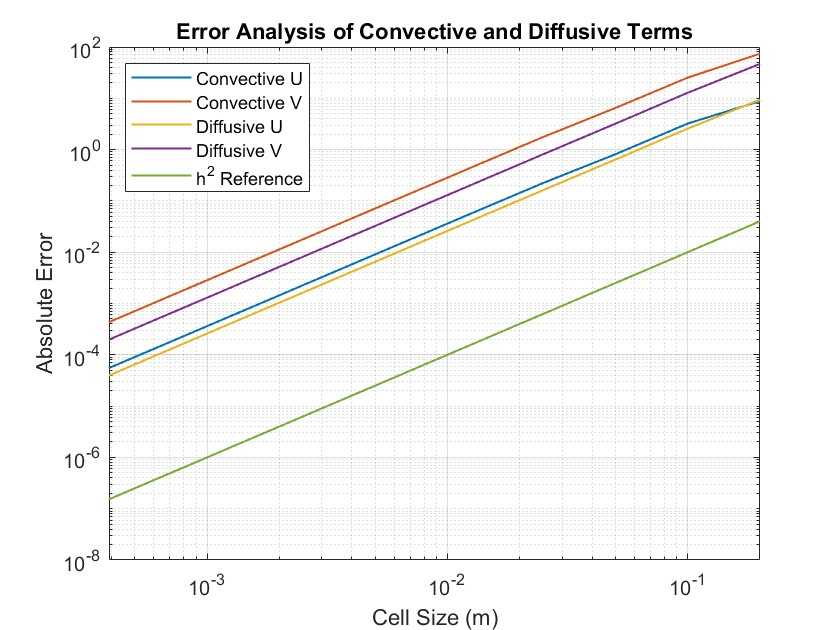
\includegraphics[width=0.7\linewidth]{imatges/PartAgraph.jpg}
    \caption{Error of computed terms}
    \label{fig:PartAError}
\end{figure}

The error lines are parallel to the $h^2$ reference, confirming second-order accuracy.